\normaltrue
\correctiontrue

%\UPSTIidClasse{11} % 11 sup, 12 spé
%\newcommand{\UPSTIidClasse}{12}

\exer{Mouvement T -- $\star$ \label{B2:13:01}}
\setcounter{question}{0}\marginnote{
\UPSTIcompetence[2]{C2-05}
\UPSTIcompetence[2]{B2-13}}

\index{Compétence C2-05}
\index{Compétence B2-13}
\index{Mécanisme à 1 translation}

\ifcorrection
\else
\marginnote{\marginnote{\textbf{Pas de corrigé pour cet exercice.}}}
\fi

\ifprof
\else
Soit le mécanisme de la figure \ref{fig_01_T:01_T_01}. On note $\vect{AB}=\lambda(t)\vect{i_0}$.
\begin{marginfigure}
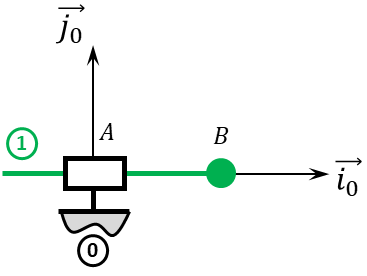
\includegraphics[width=\linewidth]{01_T_01}
\caption{\label{fig_01_T:01_T_01} 1 translation}
\end{marginfigure}
\fi

\question{Quel est le mouvement de \textbf{1} par rapport à~\textbf{0}.}
\ifprof~\\
\textbf{1} est en translation de direction $\vi{0}$ par rapport à \textbf{0}.
\else
\fi

\question{Donner l'équation paramétrique de la trajectoire du point $B$, point appartenant à \textbf{1} par rapport à~\textbf{0}.}
\ifprof~\\
On a $\vect{AB}=\lambda(t)\vect{i_0} $. La trajectoire du point $B$ est donc donnée par 
$\left\{ 
\begin{array}{l}
x_B(t) = \lambda (t) \\
y_B(t) = 0 \\
z_B(t) = 0 \\
\end{array}
\right.$ dans le repère $\repere{A}{i_0}{j_0}{z_0}$.
\else
\fi


\ifprof
\else
\marginnote{
\begin{solution}
\begin{enumerate}
\item .
\item $x_B(t) = \lambda (t)$.
\end{enumerate}
\end{solution}}
 
\marginnote{Corrigé  voir \ref{B2:13:01}.}
\fi


